% Provenance (never printed): see sources/outline_sources.md (Year 3: refraction and
% reflection seismic methods; CMP acquisition, NMO, stacking, Dix; migration in
% principle; seismic stratigraphy). Brief: sources/book5/BRIEFS.md, ch. 2. Curves from
% figdata/bachelor-3/seismic_model.py, refraction_dip.py, synthetic_seismogram.py,
% cmp_nmo.py (the Varden column, region.py); exercise and problem values in the
% Book 5 scratch calculator calc/ch02.py.
\chapter{Sismique d'exploration}\label{ch:b3:exploration-seismology}

Un navire de prospection avance lentement en ligne droite en mer, tractant un réseau de
canons à air à quelques mètres sous la surface et, derrière lui, des câbles longs de plusieurs
kilomètres, garnis d'hydrophones. Dans une campagne décrite à l'autorité de régulation,
le réseau contenait \num{5240}~pouces cubes d'air comprimé, tiré toutes les
\qty{8}{s} depuis \qty{12}{m} sous la surface, et les flûtes à azimut étroit
traînées derrière de tels navires enregistrent des déports de 8 à \qty{10}{km}.
% ledger: noaa5:wg-survey
Chaque tir envoie une impulsion sonore dans le fond marin, et chaque interface rocheuse
en profondeur renvoie un écho faible. Des semaines de traitement plus tard, un géologue fait défiler
une section dans laquelle des chenaux fluviaux enfouis, des blocs de faille basculés et
le remplissage en \omterm{def:b3:exploration-seismology:terminations}{onlap} d'un ancien bassin apparaissent comme si le sous-sol avait été mis à nu.
La sismologie à l'échelle terrestre du chapitre précédent utilisait les ondes
des séismes~; la sismique d'exploration fabrique les siennes, avec des sources dont l'instant et
le lieu sont connus avec précision, et les enregistre sur des milliers de voies. Ce
chapitre suit les échos depuis le tir jusqu'à la section~: \omterm{def:b3:exploration-seismology:surveys}{campagnes de sismique réfraction},
la réflexion d'une ondelette par une colonne stratifiée, la méthode du \omterm{def:b3:exploration-seismology:cmp}{point milieu commun}
qui transforme des échos répétés en vitesses et en image propre, la migration, qui
replace les réflecteurs à leur place, et la lecture de la section comme
stratigraphie.

\begin{recall}
À une interface entre deux milieux d'impédances acoustiques $Z_1 = \rho_1v_1$ et
$Z_2 = \rho_2v_2$, une onde plane en incidence normale est réfléchie avec le
coefficient d'amplitude $R = (Z_2 - Z_1)/(Z_2 + Z_1)$ (le volume de physique de
deuxième année, sur les ondes aux interfaces). L'onde conique, le temps d'interception et
la distance de croisement d'un profil de réfraction sur couches horizontales ont été
rencontrés au chapitre sur la Terre stratifiée du volume de première année~; les logs de sondage dans le livre~2
(année~11). La convolution $(f*g)(t) = \int f(\tau)g(t - \tau)\,\mathrm d\tau$
et la transformée de Fourier relèvent des volumes de mathématiques. Le \omterm{def:b3:seismology-imaging:ray-parameter}{paramètre de rai} et le
\omterm{def:b3:seismology-imaging:inverse}{problème inverse} linéaire sont ceux du \cref{ch:b3:seismology-imaging}.
\end{recall}

\section{Campagnes de sismique réfraction}

\begin{definition}[Campagnes de sismique réfraction et réflexion]\label{def:b3:exploration-seismology:surveys}
Une \emph{campagne de sismique réfraction}\index{campagne de sismique réfraction} enregistre, le long
d'une ligne de récepteurs, les premières arrivées issues d'une source contrôlée, et utilise les
ondes coniques qui se propagent au sommet des couches plus rapides pour en déterminer les vitesses et
profondeurs. Une \emph{campagne de sismique réflexion}\index{campagne de sismique réflexion}
enregistre l'ensemble du train d'ondes, à des déports le plus souvent inférieurs aux profondeurs
d'intérêt, et utilise les ondes réfléchies sous incidence quasi normale par les
interfaces pour imager la stratification.
\end{definition}

Sur couches horizontales, une onde conique arrive à $t = x/v_2 + t_i$, une droite
dont la pente donne la vitesse $v_2$ du réfracteur et dont le temps d'interception $t_i$
donne sa profondeur. Un réfracteur incliné fait pencher la droite~: l'onde conique tirée
dans le sens du pendage arrive de plus en plus tard, à mesure que le réfracteur s'enfonce, et paraît lente~;
tirée à contre-pendage paraît rapide. En tirant dans les deux sens le long de la même ligne, un
profil inversé sépare la vitesse du pendage.

\begin{theorem}[Réfraction sur une interface à pendage]\label{thm:b3:exploration-seismology:dipping}
Une couche de vitesse $v_1$ surmonte un réfracteur plan de vitesse $v_2 > v_1$ incliné
d'un angle $\theta$ le long du profil~; $i_c = \arcsin(v_1/v_2)$, et $h$ est la
profondeur perpendiculaire du réfracteur sous le tir. Au-delà de la
distance critique, l'onde conique arrive à
\begin{align*}
  t &= \frac{x\sin(i_c + \theta)}{v_1} + \frac{2h\cos i_c}{v_1}
  &&\text{tir dans le sens du pendage},\\
  t &= \frac{x\sin(i_c - \theta)}{v_1} + \frac{2h\cos i_c}{v_1}
  &&\text{tir à contre-pendage}.
\end{align*}
Les vitesses apparentes $v_d = v_1/\sin(i_c + \theta)$ et
$v_u = v_1/\sin(i_c - \theta)$ d'un profil inversé donnent
\[
  i_c = \tfrac12\left[\arcsin\frac{v_1}{v_d} + \arcsin\frac{v_1}{v_u}\right],\qquad
  \theta = \tfrac12\left[\arcsin\frac{v_1}{v_d} - \arcsin\frac{v_1}{v_u}\right],
  \qquad v_2 = \frac{v_1}{\sin i_c} .
\]
\end{theorem}

\begin{proof}
On tourne le repère pour que le réfracteur soit horizontal~; la surface présente alors un pendage
d'angle $\theta$, et, en tir dans le sens du pendage, la profondeur perpendiculaire sous un récepteur à
de déport $x$ est $h + x\sin\theta$, sa projection sur le réfracteur
$x\cos\theta$. Le trajet de l'onde conique descend sous l'angle critique $i_c$ jusqu'à la
normale, le long du réfracteur à $v_2$, puis remonte sous $i_c$. Son temps vaut
\[
  t = \frac{h}{v_1\cos i_c} + \frac{x\cos\theta - h\tan i_c - (h + x\sin\theta)\tan i_c}{v_2}
  + \frac{h + x\sin\theta}{v_1\cos i_c}.
\]
Avec $1/v_2 = \sin i_c/v_1$ et $1/\cos i_c - \sin i_c\tan i_c = \cos i_c$,
les termes en $h$ donnent $2h\cos i_c/v_1$ et ceux en $x$ donnent
$x(\sin i_c\cos\theta + \cos i_c\sin\theta)/v_1 = x\sin(i_c + \theta)/v_1$.
À contre-pendage, $\theta$ change de signe. Les dernières formules inversent les deux vitesses
apparentes.
\end{proof}

Les deux branches d'un profil inversé doivent donner le même temps entre les deux
points de tir, peu importe l'extrémité qui a tiré~: le \emph{temps réciproque}, un contrôle du
pointé. Deux situations mettent la méthode en échec. Une couche plus lente que celle qui la surmonte
(une inversion de vitesse) ne réfracte aucune onde conique et reste invisible~: ses roches sont
comptées dans la couche supérieure, et toute profondeur située en dessous est surestimée. Une couche
plus rapide que celle qui la surmonte mais trop mince peut ne jamais donner de première arrivée, car
l'onde conique de la couche plus profonde et plus rapide la rattrape~: une couche cachée. Une
\omterm{def:b3:exploration-seismology:surveys}{campagne de sismique réflexion} voit les deux.

\begin{omfigure}
\begin{tikzpicture}
\begin{axis}[omrecord, width=0.82\linewidth, height=0.46\linewidth,
  xmin=0, xmax=1200, ymin=0, ymax=660,
  xlabel={position le long du dispositif, depuis le tir O (\unit{m})},
  ylabel={temps (\unit{ms})}, legend pos=north west, legend cell align=left,
  legend style={font=\scriptsize}]
\addplot[gray, thick, densely dashed] table[x=x, y=tdir] {figdata/out/bachelor-3-refraction_dip-west.dat};
\addlegendentry{ondes directes ($v_1$)}
\addplot[blue!70!black, thick] table[x=x, y=thead] {figdata/out/bachelor-3-refraction_dip-west.dat};
\addlegendentry{onde conique depuis O, tir à contre-pendage}
\addplot[red!70!black, thick] table[x expr=1200-\thisrow{x}, y=thead] {figdata/out/bachelor-3-refraction_dip-east.dat};
\addlegendentry{onde conique depuis E, tir dans le sens du pendage}
\addplot[gray, thick, densely dashed, forget plot] table[x expr=1200-\thisrow{x}, y=tdir] {figdata/out/bachelor-3-refraction_dip-east.dat};
\addplot[only marks, mark=*, mark size=1.5pt] coordinates {(1200,486.13) (0,486.13)};
\node[font=\scriptsize, anchor=south east] at (axis cs:1190,530) {temps réciproque};
\end{axis}
\end{tikzpicture}

\par\smallskip{\small Une \omterm{def:b3:exploration-seismology:surveys}{campagne de sismique réfraction} inversée sur le flanc ouest de
l'anticlinal de Varden (calculée~; problème, partie I). Le réfracteur, le sommet du
calcaire, remonte de O vers E à \ang{10.8} sous un dispositif de \qty{1200}{m}~; la
craie et les argiles qui le surmontent sont regroupées en une seule couche de \qty{2.40}{km.s^{-1}}. L'onde
conique émise depuis l'O, en tir à contre-pendage, apparaît rapide (\qty{6.57}{km.s^{-1}}),
celle émise depuis l'E, dans le sens du pendage, lente (\qty{3.52}{km.s^{-1}})~; toutes deux mettent \qty{486.1}{ms}
pour traverser tout le dispositif. Les ondes coniques ne rattrapent les ondes directes
qu'à proximité de l'extrémité éloignée~: le réfracteur est profond pour un dispositif aussi court.}
\label{fig:b3:exploration-seismology:refraction}
\end{omfigure}

\section{Réflexion à incidence normale}

\begin{definition}[Ondelette sismique, ondelette de Ricker]\label{def:b3:exploration-seismology:wavelet}
Une \emph{ondelette sismique}\index{ondelette sismique} est la brève impulsion, longue de quelques dizaines
de millisecondes, que la source et le système d'enregistrement envoient dans le
sol~; chaque réflecteur en renvoie une copie, à un facteur près. La \emph{ondelette de
Ricker}\index{ondelette de Ricker} de fréquence de pic $f$ est l'impulsion à phase nulle
\[
  w(t) = \left(1 - 2\pi^2f^2t^2\right)e^{-\pi^2f^2t^2},
\]
C'est la dérivée seconde d'une gaussienne, à un signe et à un facteur d'échelle près~: un pic central et
deux lobes latéraux, de moyenne nulle et un spectre d'amplitude qui culmine en $f$.
\end{definition}

\begin{definition}[Série de réflectivité]\label{def:b3:exploration-seismology:synthetic}
La \emph{série de réflectivité}\index{série de réflectivité} d'une colonne stratifiée est la suite des
coefficients de réflexion en incidence normale $r_k$ de ses interfaces,
placés à leurs temps doubles verticaux $\tau_k = \sum_{i \le k} 2h_i/v_i$~:
$r(t) = \sum_k r_k\,\delta(t - \tau_k)$.
\end{definition}

\begin{proposition}[Le modèle convolutif]\label{prop:b3:exploration-seismology:synthetic}
Si l'on ne conserve que les réflexions primaires (sans multiples), en incidence normale, avec
aucune perte de transmission, ni atténuation ni étalement géométrique, et si l'ondelette $w$ ne
change pas avec la profondeur, la trace enregistrée est la convolution de l'ondelette avec la
\omterm{def:b3:exploration-seismology:synthetic}{série de réflectivité}~:
\[
  s(t) = \sum_k r_k\,w(t - \tau_k) = (w*r)(t) .
\]
La trace ainsi calculée à partir d'un log de sondage de vitesse et de masse volumique est le
\emph{sismogramme synthétique}\index{sismogramme synthétique} du log.
\end{proposition}

\begin{proof}
Chaque interface renvoie une copie de l'ondelette incidente, pondérée par son coefficient
et retardée de son temps double~; l'enregistrement étant linéaire, les copies s'additionnent.
La somme est la convolution de $w$ avec le train d'impulsions de Dirac pondérées
$r(t)$, puisque $w*\delta(\cdot - \tau_k) = w(\cdot - \tau_k)$.
\end{proof}

Le \omterm{prop:b3:exploration-seismology:synthetic}{sismogramme synthétique} permet de caler un forage sur une section sismique~: une
réflexion sur la section est appariée à l'interface du log qui la produit.
La colonne de Varden située sous l'axe du synclinal du problème (le modèle sismique de
ce chapitre, avec des vitesses et des masses volumiques choisies dans les fourchettes publiées pour
chaque roche)
% ledger: mavko:velocities
donne la figure ci-dessous. L'interface craie--argiles ne réfléchit que
\qty{2.8}{\percent} de l'amplitude, car la craie et les argiles ont par hasard presque la
même impédance~; le sommet du calcaire réfléchit \qty{38}{\percent},
la base du calcaire renvoie une impulsion inversée, et le socle une impulsion
forte et positive.

\begin{omfigure}
\begin{tikzpicture}
\begin{groupplot}[group style={group size=3 by 1, horizontal sep=0.45cm, y descriptions at=edge left},
  width=0.36\linewidth, height=0.6\linewidth, y dir=reverse, ymin=0.4, ymax=0.85,
  tick label style={font=\scriptsize}, label style={font=\small}, title style={font=\small}]
\nextgroupplot[title={impédance}, xlabel={\scriptsize $10^6$\,\unit{kg.m^{-2}.s^{-1}}},
  ylabel={temps double (\unit{s})}, xmin=4, xmax=14]
\addplot[black, thick] table[x=imp, y=t] {figdata/out/bachelor-3-synthetic_seismogram-log.dat};
\node[font=\tiny, anchor=west] at (axis cs:5.1,0.45) {craie};
\node[font=\tiny, anchor=west] at (axis cs:5.4,0.535) {argiles};
\node[font=\tiny, anchor=east] at (axis cs:11.6,0.62) {calcaire};
\node[font=\tiny, anchor=west] at (axis cs:7.0,0.70) {grès};
\node[font=\tiny, anchor=east] at (axis cs:13.1,0.79) {schiste};
\nextgroupplot[title={réflectivité}, xmin=-0.45, xmax=0.45, xtick={-0.4,0,0.4}]
\addplot[xcomb, red!70!black, thick, mark=*, mark size=1.2pt] table[x=r, y=t] {figdata/out/bachelor-3-synthetic_seismogram-refl.dat};
\draw[gray] (axis cs:0,0.4) -- (axis cs:0,0.85);
\nextgroupplot[title={trace synthétique}, xmin=-0.45, xmax=0.45, xtick={-0.4,0,0.4}]
\addplot[blue!70!black, thick] table[x=s, y=t] {figdata/out/bachelor-3-synthetic_seismogram-trace.dat};
\draw[gray] (axis cs:0,0.4) -- (axis cs:0,0.85);
\end{groupplot}
\end{tikzpicture}

\par\smallskip{\small \omterm{prop:b3:exploration-seismology:synthetic}{Sismogramme synthétique} de la colonne de Varden située sous l'axe
du synclinal (calculé). À gauche~: l'impédance de chaque couche en fonction du
temps double. Au centre~: la \omterm{def:b3:exploration-seismology:synthetic}{série de réflectivité}, un pic par interface (les tiges pointent
vers la droite pour une augmentation de l'impédance). À droite~: leur convolution avec une
\omterm{def:b3:exploration-seismology:wavelet}{ondelette de Ricker} à \qty{30}{Hz}. Chaque réflexion est une copie de l'ondelette~; la faible
réflexion craie--argiles, à \qty{0.488}{s}, est à peine visible.}
\label{fig:b3:exploration-seismology:synthetic}
\end{omfigure}

Jusqu'à quelle épaisseur une couche peut-elle encore être résolue par les réflexions~? Son sommet et sa base
renvoient chacun une ondelette~; lorsqu'elles se recouvrent, elles interfèrent.

\begin{definition}[Épaisseur d'accord]\label{def:b3:exploration-seismology:resolution}
L'\emph{épaisseur d'accord}\index{epaisseur d'accord@épaisseur d'accord} d'un banc est l'épaisseur
à laquelle les réflexions de son sommet et de sa base, de signes opposés, interfèrent
le plus constructivement, de sorte que l'amplitude composite soit maximale. Les bancs plus minces
ne sont pas résolus~: leur sommet et leur base ne peuvent plus être pointés séparément, et
l'amplitude décroît proportionnellement à l'épaisseur.
\end{definition}

\begin{proposition}[Règle du quart de longueur d'onde]\label{prop:b3:exploration-seismology:tuning}
Pour une ondelette de période dominante $T$ dans un banc de vitesse $v$, avec des coefficients de réflexion
$+R$ à son sommet et $-R$ à sa base, la réflexion composite est
maximale lorsque l'épaisseur du banc vaut $b = \lambda/4$, où $\lambda = vT$~; pour
$b \ll \lambda/4$, son amplitude est proportionnelle à $b$.
\end{proposition}

\begin{proof}
On représente l'ondelette par son harmonique dominante $\cos(2\pi t/T)$. Les deux
réflexions valent $R\cos(2\pi t/T) - R\cos(2\pi(t - \Delta t)/T)$ avec
$\Delta t = 2b/v$, dont l'amplitude vaut $2R|\sin(\pi\Delta t/T)|$~: elle est maximale pour
$\Delta t = T/2$, soit $b = vT/4$~; pour $\Delta t$ petit, elle vaut environ
$2\pi R\Delta t/T = 4\pi Rb/\lambda$.
\end{proof}

Une \omterm{def:b3:exploration-seismology:wavelet}{ondelette de Ricker} n'est pas un harmonique, et son \omterm{def:b3:exploration-seismology:resolution}{épaisseur d'accord}, lue sur le modèle en biseau de la figure ci-dessous,
est un peu plus petite que le quart de la longueur d'onde
à la fréquence de pic~: \qty{19.5}{m} pour \qty{30}{Hz} dans une roche de
\qty{3000}{m.s^{-1}}, soit $\lambda/4 = \qty{25}{m}$. Les données sismiques contiennent rarement
beaucoup d'énergie au-delà de quelques dizaines de hertz provenant de profondeurs kilométriques, car les
roches absorbent les hautes fréquences~; les bancs d'épaisseur inférieure à environ \qty{20}{m} apparaissent
comme une réflexion unique.

\begin{omfigure}
\begin{tikzpicture}
\begin{axis}[omrecord, width=0.74\linewidth, height=0.42\linewidth,
  xmin=0, xmax=80, ymin=0, ymax=1.8,
  xlabel={épaisseur du banc $b$ (\unit{m})}, ylabel={amplitude au pic / $R$}]
\addplot[blue!70!black, thick] table[x=b, y expr=2*\thisrow{amp}] {figdata/out/bachelor-3-synthetic_seismogram-wedge.dat};
\draw[red!70!black, densely dashed] (axis cs:19.5,0) -- (axis cs:19.5,1.6);
\node[font=\scriptsize, anchor=south, red!70!black] at (axis cs:19.5,1.6) {épaisseur d'accord, \qty{19.5}{m}};
\draw[gray, densely dotted] (axis cs:25,0) -- (axis cs:25,1.6);
\node[font=\scriptsize, anchor=west, gray!40!black] at (axis cs:25.5,0.3) {$\lambda/4 = \qty{25}{m}$};
\draw[gray] (axis cs:0,1) -- (axis cs:80,1);
\node[font=\scriptsize, anchor=south east] at (axis cs:79,1) {deux ondelettes séparées};
\end{axis}
\end{tikzpicture}

\par\smallskip{\small Le modèle en biseau (calculé)~: un banc de
\qty{3000}{m.s^{-1}}, avec des coefficients de réflexion $+R$ à son sommet et $-R$ à
sa base, imagé avec une \omterm{def:b3:exploration-seismology:wavelet}{ondelette de Ricker} de \qty{30}{Hz}. L'amplitude au pic de la
réflexion composite, rapportée à une réflexion unique de coefficient $R$, croît linéairement depuis zéro pour des bancs très
minces, atteint son maximum à l'\omterm{def:b3:exploration-seismology:resolution}{épaisseur d'accord} et se stabilise au niveau de deux
ondelettes séparées pour les bancs épais.}
\label{fig:b3:exploration-seismology:wedge}
\end{omfigure}

Latéralement, la résolution est fixée par la largeur du réflecteur qui renvoie
l'énergie en phase.

\begin{definition}[Zone de Fresnel]\label{def:b3:exploration-seismology:fresnel}
La \emph{zone de Fresnel}\index{zone de Fresnel} (première) d'un réflecteur, pour une
source et un récepteur confondus à la hauteur $z$ au-dessus de lui, est le disque du réflecteur
autour du point d'incidence normale à partir duquel le trajet aller-retour est plus long que le
trajet normal de moins d'une demi-longueur d'onde~: ses réflexions arrivent en phase et
construisent ensemble la réflexion enregistrée.
\end{definition}

\begin{proposition}[Rayon de la zone de Fresnel]\label{prop:b3:exploration-seismology:fresnel}
La première \omterm{def:b3:exploration-seismology:fresnel}{zone de Fresnel} a pour rayon
$r_F = \sqrt{\lambda z/2 + \lambda^2/16} \approx \sqrt{\lambda z/2}$ pour
$\lambda \ll z$.
\end{proposition}

\begin{proof}
Un point du réflecteur situé à la distance $r$ du point d'incidence normale est
à la distance $\sqrt{z^2 + r^2}$ de la source. Le surplus de trajet aller-retour vaut
$2(\sqrt{z^2 + r^2} - z)$~; en l'égalant à $\lambda/2$, on obtient
$\sqrt{z^2 + r^2} = z + \lambda/4$, d'où $r^2 = \lambda z/2 + \lambda^2/16$.
\end{proof}

À une profondeur de \qty{1}{km}, avec $\lambda = \qty{100}{m}$, la \omterm{def:b3:exploration-seismology:fresnel}{zone de Fresnel}
fait \qty{225}{m} de rayon~: les structures plus étroites que cela sont floues, sauf si
la migration (ci-dessous) resserre la zone.

\begin{omfigure}
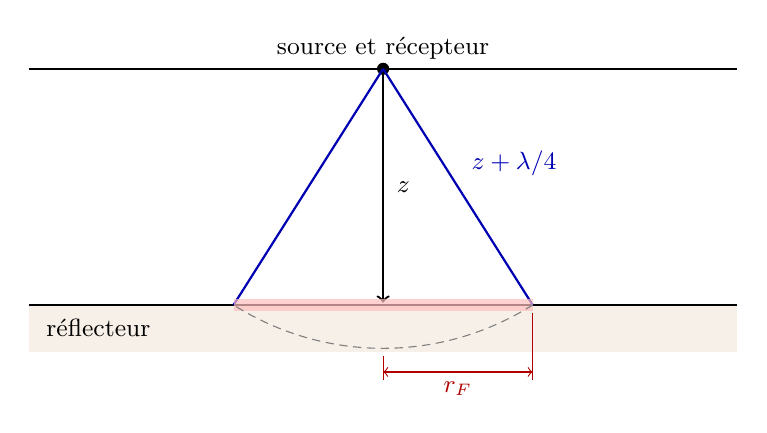
\begin{tikzpicture}[font=\small, x=1cm, y=1cm]
\fill[brown!12] (-4.5,-3.6) rectangle (4.5,-3.0);
\draw[thick] (-4.5,-3.0) -- (4.5,-3.0);
\node[anchor=north west] at (-4.4,-3.05) {réflecteur};
\draw[thick] (-4.5,0) -- (4.5,0);
\fill (0,0) circle (2.2pt) node[above] {source et récepteur};
\draw[->, thick] (0,0) -- (0,-2.97);
\node[anchor=west] at (0.05,-1.5) {$z$};
\draw[blue!70!black, thick] (0,0) -- (1.9,-3.0);
\draw[blue!70!black, thick] (0,0) -- (-1.9,-3.0);
\node[anchor=west, blue!70!black] at (1.0,-1.2) {$z + \lambda/4$};
\fill[red!25, opacity=0.7] (-1.9,-3.08) rectangle (1.9,-2.92);
\draw[red!70!black] (0,-3.65) -- (0,-3.95) (1.9,-3.1) -- (1.9,-3.95);
\draw[<->, red!70!black] (0,-3.85) -- (1.9,-3.85) node[midway, below] {$r_F$};
\draw[gray, densely dashed] (-57.6:3.55) arc (-57.6:-122.4:3.55);
\end{tikzpicture}

\par\smallskip{\small La première \omterm{def:b3:exploration-seismology:fresnel}{zone de Fresnel} (schéma)~: la partie du
réflecteur dont la distance à une source et un récepteur confondus dépasse la
distance normale $z$ de moins de $\lambda/4$ (arc en pointillés~: la sphère de rayon
$z + \lambda/4$), de sorte que le surplus de trajet aller-retour soit inférieur à une demi-longueur d'onde
et que ses échos arrivent en phase. L'échelle de $\lambda$ est exagérée.}
\label{fig:b3:exploration-seismology:fresnel}
\end{omfigure}

\section{Acquisition et traitement en point milieu commun}

Un écho isolé est trop faible pour être distingué du bruit. Les \omterm{def:b3:exploration-seismology:surveys}{campagnes de sismique réflexion} enregistrent donc
chaque point du sous-sol un grand nombre de fois, avec différents couples source--récepteur,
et en additionnent les enregistrements.

\begin{definition}[Point milieu commun, ordre de couverture]\label{def:b3:exploration-seismology:cmp}
Pour une source en $x_s$ et un récepteur en $x_r$ sur une ligne, le point milieu vaut
$(x_s + x_r)/2$ et le déport $x = |x_r - x_s|$. On appelle \emph{point
milieu commun}\index{point milieu commun} (CMP) l'ensemble des traces, issues de tous les tirs, qui ont le même point milieu~;
sur des couches planes, toutes se réfléchissent sur le même
point du sous-sol. L'\emph{ordre de couverture}\index{ordre de couverture}
est le nombre de traces d'une collection. Avec $N$ canaux à
l'intervalle $\Delta g$ entre récepteurs et un tir tous les $\Delta s$ le long de la ligne, l'ordre
de couverture vaut $N\Delta g/(2\Delta s)$.
\end{definition}

\begin{omfigure}
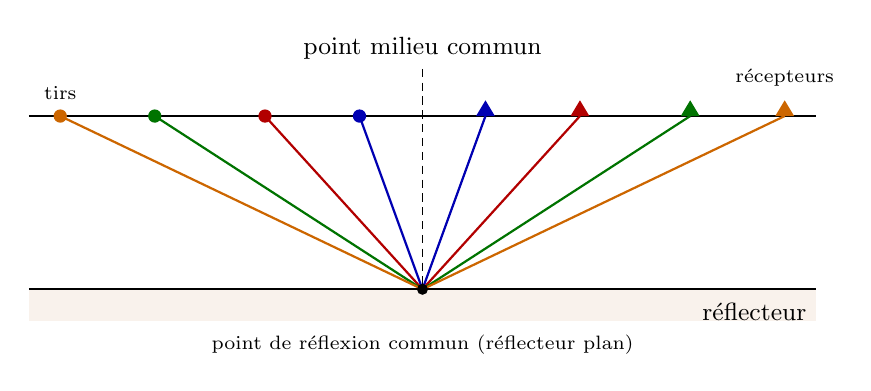
\begin{tikzpicture}[font=\small, x=1cm, y=1cm]
\draw[thick] (-5,0) -- (5,0);
\fill[brown!10] (-5,-2.6) rectangle (5,-2.2);
\draw[thick] (-5,-2.2) -- (5,-2.2);
\node[anchor=north east] at (5,-2.25) {réflecteur};
\foreach \off/\col in {0.8/blue!70!black, 2.0/red!70!black, 3.4/green!45!black, 4.6/orange!80!black} {
  \draw[\col, thick] (-\off,0) -- (0,-2.2) -- (\off,0);
  \fill[\col] (-\off,0) circle (2.4pt);
  \fill[\col] (\off-0.12,0) -- (\off+0.12,0) -- (\off,0.2) -- cycle;
}
\fill (0,-2.2) circle (2pt);
\draw[densely dashed] (0,0.6) -- (0,-2.2);
\node[anchor=south] at (0,0.6) {point milieu commun};
\node[anchor=north, align=center, font=\scriptsize] at (0,-2.65) {point de réflexion commun (réflecteur plan)};
\node[anchor=south, font=\scriptsize] at (-4.6,0.08) {tirs};
\node[anchor=south, font=\scriptsize] at (4.6,0.25) {récepteurs};
\end{tikzpicture}

\par\smallskip{\small Géométrie à \omterm{def:b3:exploration-seismology:cmp}{point milieu commun} (schématique)~: quatre couples source--récepteur
(points, triangles) de déports différents partagent le même point milieu~; sur un
réflecteur plan, toutes se réfléchissent au même point situé sous lui. Leurs traces forment une
collection d'\omterm{def:b3:exploration-seismology:cmp}{ordre de couverture} quatre.}
\label{fig:b3:exploration-seismology:cmp}
\end{omfigure}

\begin{theorem}[Retard normal]\label{thm:b3:exploration-seismology:nmo}
Dans une couche de vitesse $v$ surmontant un réflecteur plan, au temps double vertical
$t_0$, la réflexion enregistrée au déport $x$ arrive en
\[
  t(x)^2 = t_0^2 + \frac{x^2}{v^2},
\]
il s'agit d'une hyperbole dans le plan $(x, t)$. Le retard $\Delta t = t(x) - t_0$ est le
\emph{retard normal}\index{retard normal}~; pour $x \ll vt_0$,
$\Delta t \approx x^2/(2v^2t_0)$.
\end{theorem}

\begin{proof}
Le trajet de la réflexion va de la source au point de réflexion sous le
point milieu, puis remonte jusqu'au récepteur~: deux branches de longueur
$\sqrt{(vt_0/2)^2 + (x/2)^2}$. D'où $t = (2/v)\sqrt{(vt_0/2)^2 + (x/2)^2}$ et
$t^2 = t_0^2 + x^2/v^2$. Ensuite $t - t_0 = (t^2 - t_0^2)/(t + t_0) \approx
x^2/(2v^2t_0)$.
\end{proof}

Sur plusieurs couches, le temps de réflexion n'est plus exactement hyperbolique, mais il
l'est presque aux petits déports, avec une vitesse qui est une moyenne pondérée des
couches.

\begin{definition}[Sommation, vitesses quadratiques moyennes et d'intervalle]\label{def:b3:exploration-seismology:velocities}
La \emph{vitesse d'intervalle}\index{vitesse d'intervalle} $v_i$ d'une couche est sa
propre vitesse~; avec $\Delta t_i = 2h_i/v_i$ le temps double à travers elle, la
\emph{vitesse quadratique moyenne}\index{vitesse quadratique moyenne} jusqu'à la base
de la couche $n$ est
\[
  V_{\text{qm},n} = \left(\frac{\sum_{i\le n}v_i^2\,\Delta t_i}{\sum_{i\le n}\Delta t_i}\right)^{1/2}.
\]
La \emph{vitesse de sommation}\index{vitesse de sommation} d'une réflexion est la
vitesse $V$ de l'hyperbole $t^2 = t_0^2 + x^2/V^2$ qui ajuste au mieux ses temps dans une
collection CMP.
\end{definition}

\begin{proposition}[Vitesse de sommation aux petits déports]\label{prop:b3:exploration-seismology:rms}
Sur des couches planes, $t(x)^2 = t_0^2 + x^2/V_{\text{qm}}^2 + O(x^4)$~: aux petits
déports, la \omterm{def:b3:exploration-seismology:velocities}{vitesse de sommation} est la \omterm{def:b3:exploration-seismology:velocities}{vitesse quadratique moyenne}.
\end{proposition}

\begin{proof}
Pour le \omterm{def:b3:seismology-imaging:ray-parameter}{paramètre de rai} $p$, $x = \sum_i 2h_i\tan\varphi_i$ et
$t = \sum_i 2h_i/(v_i\cos\varphi_i)$, avec $\sin\varphi_i = pv_i$. Au deuxième
ordre en $p$, $\tan\varphi_i \approx pv_i$ et $1/\cos\varphi_i \approx 1 +
p^2v_i^2/2$, donc $x \approx p\sum v_i^2\Delta t_i = pV_{\text{qm}}^2t_0$ et
$t \approx t_0 + \tfrac12p^2V_{\text{qm}}^2t_0$. Ensuite
$t^2 \approx t_0^2 + p^2V_{\text{qm}}^2t_0^2 = t_0^2 + x^2/V_{\text{qm}}^2$, les
termes négligés étant d'ordre $p^4$, soit $x^4$.
\end{proof}

\begin{theorem}[Équation de Dix]\label{thm:b3:exploration-seismology:dix}
Si $V_{n-1}$ et $V_n$ sont les \omterm{def:b3:exploration-seismology:velocities}{vitesses quadratiques moyennes} au sommet et à la base de la
couche $n$, aux temps doubles $t_{n-1}$ et $t_n$, la \omterm{def:b3:exploration-seismology:velocities}{vitesse d'intervalle} de la
couche est donnée par l'\emph{équation de Dix}\index{equation de Dix@équation de Dix}
\[
  v_n^2 = \frac{V_n^2t_n - V_{n-1}^2t_{n-1}}{t_n - t_{n-1}} ,
\]
et son épaisseur est $h_n = v_n(t_n - t_{n-1})/2$.
\end{theorem}

\begin{proof}
Par définition $V_n^2t_n = \sum_{i\le n}v_i^2\Delta t_i$ et $V_{n-1}^2t_{n-1}
= \sum_{i\le n-1}v_i^2\Delta t_i$. Leur différence vaut $v_n^2\Delta t_n$, avec
$\Delta t_n = t_n - t_{n-1}$.
\end{proof}

L'analyse de vitesse parcourt chaque collection à la recherche de l'hyperbole qui ajuste au mieux
l'énergie~: pour chaque essai $t_0$ et $V$, les traces sont sommées le long de la courbe, et
une mesure de cohérence (la semblance) est cartographiée~; l'analyste en retient les maxima,
réflecteur par réflecteur, pour construire une fonction de vitesse. La correction de \omterm{thm:b3:exploration-seismology:nmo}{retard normal}
(NMO) décale chaque échantillon de chaque trace de $t(x)$ à $t_0$, aplanissant les
réflexions, puis les traces de chaque collection sont additionnées.

\begin{definition}[Sommation (sismique)]\label{def:b3:exploration-seismology:stack}
La \emph{sommation}\index{sommation (sismique)} est la somme, après la
correction de \omterm{thm:b3:exploration-seismology:nmo}{retard normal}, des traces d'une collection CMP en une seule trace
placée au point milieu. Les traces sommées, côte à côte le long de la ligne, forment
la section sommée, image des réflecteurs en temps double.
\end{definition}

\begin{proposition}[Gain d'une sommation]\label{prop:b3:exploration-seismology:sqrtN}
Si les $N$ traces d'une collection portent le même signal de réflexion et un bruit indépendant
de même écart-type $\sigma$, leur moyenne porte le même signal
et un bruit d'écart-type $\sigma/\sqrt N$~: la \omterm{def:b3:exploration-seismology:stack}{sommation} augmente le
rapport signal sur bruit d'un facteur $\sqrt N$.
\end{proposition}

\begin{proof}
La variance d'une somme de $N$ variables indépendantes est la somme de leurs
variances, soit $N\sigma^2$~; divisée par $N^2$, la moyenne a pour variance
$\sigma^2/N$ (l'écart-type de la moyenne, rappelé des
volumes de mathématiques).
\end{proof}

\begin{omfigure}
\begin{tikzpicture}
\begin{groupplot}[group style={group size=2 by 1, horizontal sep=0.5cm, y descriptions at=edge left},
  width=0.52\linewidth, height=0.56\linewidth, y dir=reverse, ymin=0.4, ymax=0.92,
  xmin=-150, xmax=2150, tick label style={font=\scriptsize}, title style={font=\small},
  xlabel={\scriptsize déport (\unit{m})}]
\nextgroupplot[title={(a) collection CMP}, ylabel={temps double (\unit{s})}]
\addplot[black, very thin, unbounded coords=jump] table[x=x, y=t] {figdata/out/bachelor-3-cmp_nmo-gather-raw.dat};
\nextgroupplot[title={(b) après correction de retard normal}]
\addplot[black, very thin, unbounded coords=jump] table[x=x, y=t] {figdata/out/bachelor-3-cmp_nmo-gather-nmo.dat};
\end{groupplot}
\end{tikzpicture}

\par\smallskip{\small Une collection CMP synthétique sous l'axe du synclinal de la
ligne de Varden (calculée par tracé de rais exact à travers la colonne à couches planes~; \omterm{def:b3:exploration-seismology:wavelet}{ondelette de Ricker} à
30~Hz~; sans bruit). (a) Les quatre réflexions (toit du schiste, toit
et base du calcaire, toit du socle) s'incurvent vers le bas avec le déport, le long
d'hyperboles presque parfaites. (b) Après la correction de \omterm{thm:b3:exploration-seismology:nmo}{retard normal}, avec les \omterm{def:b3:exploration-seismology:velocities}{vitesses de sommation}
ajustées sur les déports allant jusqu'à \qty{600}{m}, les réflexions sont plates jusqu'à
environ \qty{1}{km}~; au-delà, les temps vrais s'écartent de l'hyperbole, la
correction les laisse courbées et les ondelettes sont étirées~; en traitement, les
traces lointaines étirées des réflexions superficielles sont coupées avant la
\omterm{def:b3:exploration-seismology:stack}{sommation}.}
\label{fig:b3:exploration-seismology:gather}
\end{omfigure}

\begin{omfigure}
\begin{tikzpicture}
\begin{axis}[omrecord, width=0.72\linewidth, height=0.46\linewidth,
  xmin=0.4, xmax=0.78, ymin=2000, ymax=5000,
  xlabel={temps double $t_0$ (\unit{s})}, ylabel={vitesse (\unit{m.s^{-1}})},
  legend cell align=left, legend columns=2,
  legend style={font=\scriptsize, at={(0.5,-0.24)}, anchor=north}]
\addplot[gray, thick, const plot mark right] table[x=t0, y=vint] {figdata/out/bachelor-3-cmp_nmo-vel.dat};
\addlegendentry{vitesse d'intervalle du modèle}
\addplot[gray, thick, forget plot] coordinates {(0.4,2500) (0.487847,2500)};
\addplot[blue!70!black, thick, mark=*, mark size=1.5pt] table[x=t0, y=vrms] {figdata/out/bachelor-3-cmp_nmo-vel.dat};
\addlegendentry{vitesse quadratique moyenne}
\addplot[red!70!black, only marks, mark=square*, mark size=1.6pt] table[x=t0, y=vstack] {figdata/out/bachelor-3-cmp_nmo-vel.dat};
\addlegendentry{vitesse de sommation (déports jusqu'à \qty{600}{m})}
\addplot[green!45!black, only marks, mark=triangle*, mark size=2pt] table[x=t0, y=vdix] {figdata/out/bachelor-3-cmp_nmo-vel.dat};
\addlegendentry{vitesse d'intervalle de Dix}
\end{axis}
\end{tikzpicture}

\par\smallskip{\small Vitesses sous l'axe du synclinal (calculées). La \omterm{def:b3:exploration-seismology:velocities}{vitesse
quadratique moyenne}, une moyenne pondérée, varie lentement~; les \omterm{def:b3:exploration-seismology:velocities}{vitesses de sommation}
de la collection s'en rapprochent. Appliquée à celles-ci, l'\omterm{thm:b3:exploration-seismology:dix}{équation de Dix} retrouve
la \omterm{def:b3:exploration-seismology:velocities}{vitesse d'intervalle} de chaque couche (le trait en escalier tracé à la base de chacune) à
quelques pour cent près, l'erreur croissant dans le calcaire mince et rapide.}
\label{fig:b3:exploration-seismology:velocities}
\end{omfigure}

\begin{omfigure}
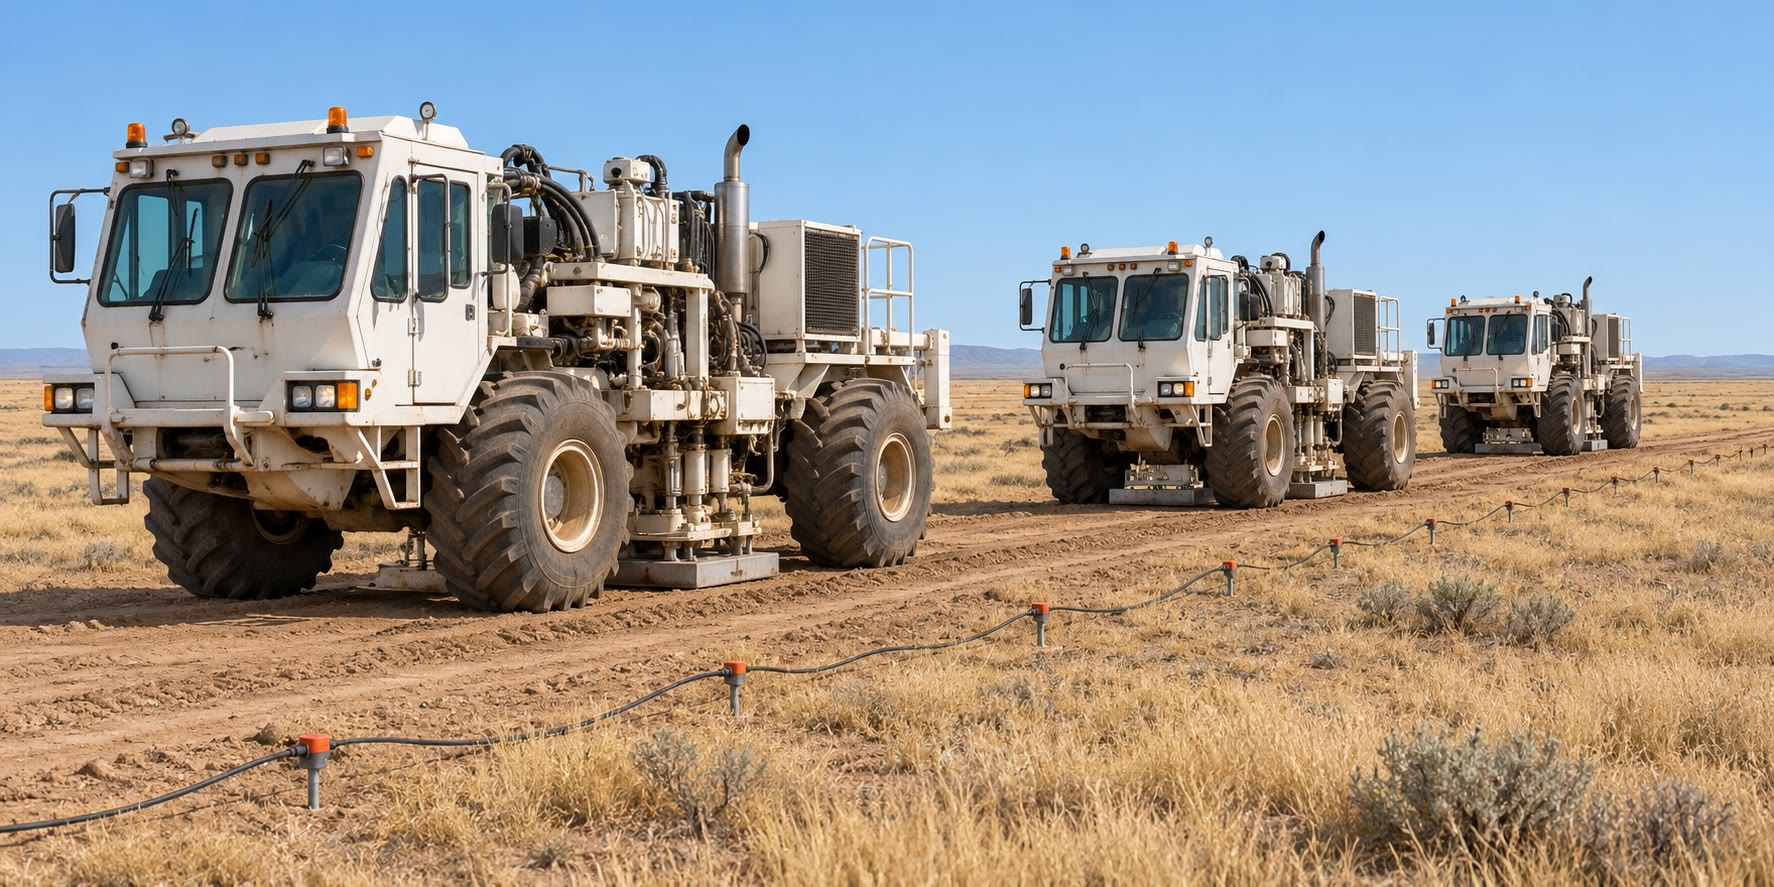
\includegraphics[width=0.62\linewidth]{images/book5/ai/b3-vibroseis.jpg}

\par\smallskip{\small Camions vibreurs sur une ligne de prospection terrestre~: au lieu
d'une explosion, chaque camion appuie une lourde plaque sur le sol et la fait vibrer
avec un balayage de fréquences pendant plusieurs secondes~; les longs enregistrements sont
comprimés en impulsions courtes par corrélation avec le balayage (Illustration générée par IA.)}
\label{fig:b3:exploration-seismology:vibroseis}
\end{omfigure}

\section{Migration}

Une section sommée montre chaque réflexion sous le point milieu où elle a été
enregistrée, au temps qu'elle a mis pour revenir. Pour un réflecteur plan, c'est
là qu'elle se trouve. Pour un réflecteur incliné, ce n'est pas le cas~: l'écho enregistré en un point de surface
provient du point du réflecteur le plus proche de lui, situé vers le haut du pendage, et non
à la verticale. Les points comme les extrémités de failles, qui diffusent l'énergie dans toutes les
directions, apparaissent sous forme d'hyperboles.

\begin{definition}[Migration sismique]\label{def:b3:exploration-seismology:migration}
La \emph{migration sismique}\index{migration sismique} est l'étape de traitement qui
déplace les réflexions d'une section sismique vers les positions des réflecteurs
qui les ont produites~: elle restaure les pendages et positions vrais des réflecteurs inclinés
réflecteurs et ramène les hyperboles de diffraction des diffuseurs ponctuels sur
leurs sommets. Réalisée avec un modèle de vitesses en temps, elle donne une
section migrée en temps~; avec un modèle en profondeur, une image en profondeur.
\end{definition}

\begin{theorem}[Pendage sur une section à déport nul]\label{thm:b3:exploration-seismology:dip}
Dans un milieu de vitesse $v$, un réflecteur plan de pendage $\theta$ dans le plan de la
section apparaît sur la section à déport nul, tracée en profondeur $vt/2$
verticalement sous chaque point d'enregistrement, comme une ligne de pendage apparent $\theta_a$
avec
\[
  \tan\theta_a = \sin\theta .
\]
La réflexion enregistrée au point $x$ provient du point du réflecteur situé à
une distance $(vt/2)\sin\theta$ vers le haut du pendage, du point situé à la verticale de $x$.
\end{theorem}

\begin{proof}
Le rai à déport nul est normal au réflecteur, donc le temps enregistré en $x$ vaut
$t = 2d(x)/v$, où $d(x)$ est la distance de $x$ au plan. Cette distance
croît de $\sin\theta$ pour chaque unité de $x$ dans le sens du pendage, donc la profondeur tracée
$vt/2 = d(x)$ a pour pente $\sin\theta$. Le pied de la normale issue de $x$
au plan se trouve à la distance horizontale $d\sin\theta$ de $x$, du côté
situé vers le haut du pendage.
\end{proof}

Comme $\tan\theta_a = \sin\theta < \tan\theta$, une section non migrée montre toujours
des pendages plus faibles que les vrais, et elle ne peut pas montrer des pendages supérieurs
à \ang{45}. Un diffuseur ponctuel de profondeur $z$ sous le point $x_0$ renvoie en
$x$ le temps à déport nul $t(x) = (2/v)\sqrt{z^2 + (x - x_0)^2}$~: une hyperbole dont
le sommet se trouve à la verticale du point~: c'est la diffraction. La migration sous sa forme la plus simple,
la \omterm{def:b3:exploration-seismology:stack}{sommation} de diffraction, additionne chaque section le long de l'hyperbole de diffraction de
chaque diffuseur possible et place la somme au sommet~: les réflecteurs, qui sont
des lignes continues de diffuseurs, ressortent à leur vraie place, et les
diffractions se resserrent en un point.

\begin{omfigure}
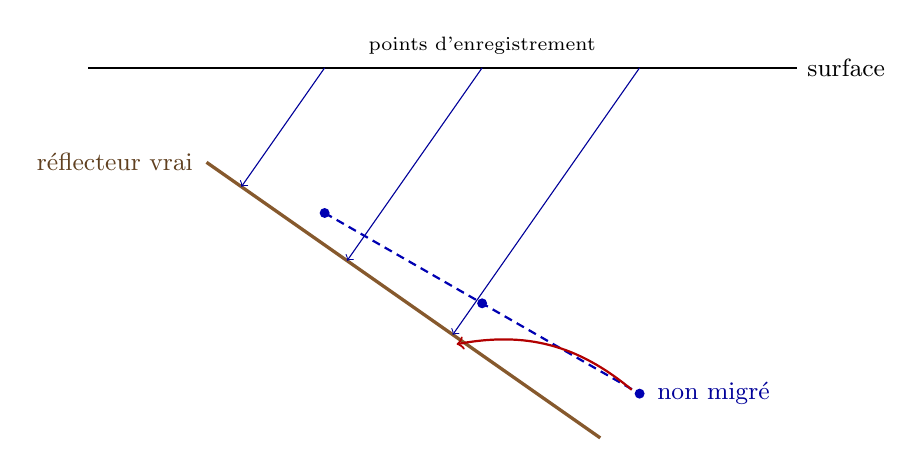
\begin{tikzpicture}[font=\small, x=1cm, y=1cm]
\draw[thick] (-0.5,0) -- (8.5,0) node[right] {surface};
% true reflector, dip 35 deg, rising to the left
\draw[very thick, brown!70!black] (1.0,-1.2) -- (6.0,-4.70);
\node[brown!50!black, anchor=east] at (0.95,-1.2) {réflecteur vrai};
% zero-offset normal rays from x = 2, 4, 6
\foreach \x in {2.5, 4.5, 6.5} {
  % distance from (x,0) to the line through (1,-1.2) dir (cos35,-sin35): normal n=(sin35,cos35)
  \pgfmathsetmacro{\dd}{abs(0.5736*(\x-1.0) + 0.8192*(0+1.2))}
  \draw[blue!60!black, ->] (\x,0) -- ++({-0.5736*\dd},{-0.8192*\dd});
  \fill[blue!70!black] (\x,{-\dd}) circle (1.8pt);
}
% apparent reflector through the plotted points
\pgfmathsetmacro{\da}{abs(0.5736*1.5 + 0.8192*1.2)}
\pgfmathsetmacro{\db}{abs(0.5736*5.5 + 0.8192*1.2)}
\draw[blue!70!black, thick, densely dashed] (2.5,{-\da}) -- (6.5,{-\db});
\node[blue!60!black, anchor=west] at (6.6,{-\db}) {non migré};
\node[anchor=south, font=\scriptsize] at (4.5,0.05) {points d'enregistrement};
\draw[->, red!70!black, thick] (6.4,{-\db+0.05}) to[bend right=25] ({6.5-0.5736*\db+0.05},{-0.8192*\db-0.12});
\end{tikzpicture}

\par\smallskip{\small Migration d'un réflecteur incliné (schéma, pendage vrai
\ang{35}). Le rai à déport nul en chaque point d'enregistrement est normal au
réflecteur, de sorte que son écho provient de l'amont-pendage~; reporté à la verticale du point,
à la profondeur $vt/2$, le réflecteur apparaît moins incliné (tireté~: $\tan\theta_a =
\sin\theta$, ici \ang{29.8}) et décalé vers l'aval-pendage. La migration (flèche rouge) le ramène à sa place.}
\label{fig:b3:exploration-seismology:migration}
\end{omfigure}

\section{Stratigraphie sismique}

Une section migrée est une image de la stratification, et on peut la lire
comme une stratigraphie~: les réflexions suivent les surfaces de stratification, qui sont
des lignes de même temps, de sorte que leur géométrie enregistre la façon dont le bassin s'est comblé.

\begin{definition}[Stratigraphie sismique, faciès sismiques]\label{def:b3:exploration-seismology:seismic-stratigraphy}
La \emph{stratigraphie sismique}\index{stratigraphie sismique} est l'interprétation
de la stratigraphie et de l'histoire de remplissage d'un bassin à partir de la géométrie
de ses réflexions sismiques. Un \emph{faciès sismique}\index{faciès sismique} est une
unité tridimensionnelle de réflexions dont le caractère (continuité, amplitude,
fréquence, géométrie interne~: parallèle, divergente, sigmoïde, chaotique, en dôme) se
distingue de celui de ses voisines et s'interprète comme un milieu
de dépôt.
\end{definition}

\begin{definition}[Terminaisons de réflexions]\label{def:b3:exploration-seismology:terminations}
Une \emph{terminaison de réflexion}\index{terminaison de réflexion} est la fin d'une
réflexion contre une autre. \emph{Onlap}\index{onlap}~: une réflexion initialement horizontale
vient buter contre une surface qui se redresse plus fortement, les couches plus jeunes
s'appuyant sur une pente plus ancienne. \emph{Downlap}\index{downlap}~: une réflexion inclinée
se termine vers l'aval-pendage contre une surface plus douce, les pieds des couches progradantes
reposant sur le fond d'un bassin. \emph{Toplap}\index{toplap}~: des réflexions inclinées
se terminent vers l'amont-pendage contre une surface sus-jacente, avec peu d'érosion, les sommets
des couches progradantes rejoignant le niveau de la mer. \emph{Troncature
d'érosion}\index{troncature d'érosion}~: des réflexions se terminent vers l'amont-pendage
contre une surface sus-jacente qui les coupe, une discordance.
\end{definition}

\begin{omfigure}
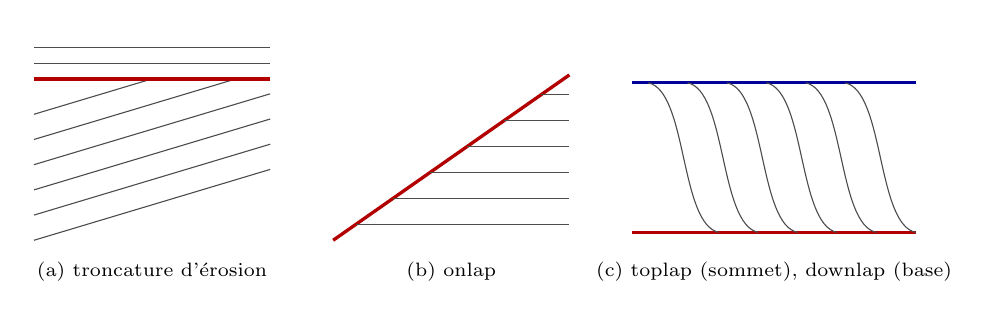
\begin{tikzpicture}[font=\scriptsize, x=1cm, y=1cm]
% erosional truncation: tilted beds cut by an unconformity
\begin{scope}
\foreach \k in {0,...,5} {\draw[gray!60!black] (0,{-2.3+0.32*\k}) -- (3.0,{-1.4+0.32*\k-0.25*0});}
\fill[white] (0,-0.25) -- (3.2,-0.25) -- (3.2,0.4) -- (0,0.4) -- cycle;
\draw[very thick, red!70!black] (0,-0.25) -- (3.0,-0.25);
\foreach \k in {0,1} {\draw[gray!60!black] (0,{-0.05+0.2*\k}) -- (3.0,{-0.05+0.2*\k});}
\node[anchor=north] at (1.5,-2.45) {(a) troncature d'érosion};
\end{scope}
% onlap
\begin{scope}[xshift=3.8cm]
\draw[very thick, red!70!black] (0,-2.3) -- (3.0,-0.2);
\foreach \k in {0,...,5} {\pgfmathsetmacro{\y}{-2.1+0.33*\k} \pgfmathsetmacro{\xe}{(\y+2.3)/0.7} \draw[gray!60!black] (\xe,\y) -- (3.0,\y);}
\node[anchor=north] at (1.5,-2.45) {(b) onlap};
\end{scope}
% downlap and toplap: clinoforms
\begin{scope}[xshift=7.6cm]
\draw[very thick, red!70!black] (0,-2.2) -- (3.6,-2.2);
\draw[very thick, blue!60!black] (0,-0.3) -- (3.6,-0.3);
\foreach \k in {0,...,5} {\draw[gray!60!black] ({0.2+0.5*\k},-0.3) .. controls ({0.7+0.5*\k},-0.4) and ({0.6+0.5*\k},-2.1) .. ({1.1+0.5*\k},-2.2);}
\node[anchor=north] at (1.8,-2.45) {(c) toplap (sommet), downlap (base)};
\end{scope}
\end{tikzpicture}

\par\smallskip{\small \omterm{def:b3:exploration-seismology:terminations}{Terminaisons de réflexions} (coupes schématiques, réflexions grises,
surfaces de terminaison en couleur). (a) Réflexions inclinées tronquées par une
discordance. (b) Réflexions horizontales venant buter contre une pente plus ancienne. (c) Couches
inclinées d'un prisme progradant se terminant vers l'amont-pendage contre la surface
sus-jacente (\omterm{def:b3:exploration-seismology:terminations}{toplap}) et vers l'aval-pendage sur le fond du bassin (\omterm{def:b3:exploration-seismology:terminations}{downlap}).}
\label{fig:b3:exploration-seismology:terminations}
\end{omfigure}

Les terminaisons marquent les surfaces qui bornent des séquences de couches
génétiquement liées~; les cartographier à l'échelle d'un bassin et les relier aux variations
du niveau marin relatif relève de la stratigraphie séquentielle, objet du
\cref{ch:b3:sequence-stratigraphy}. Une section sismique d'une marge passive montre
typiquement des prismes de réflexions progradant vers le large, en \omterm{def:b3:exploration-seismology:terminations}{downlap} sur le
plancher profond, coiffés de \omterm{def:b3:exploration-seismology:terminations}{toplap}, et enfouis vers la terre sous des couches en \omterm{def:b3:exploration-seismology:terminations}{onlap} déposées
lorsque la mer est remontée.

\begin{inthefield}[Une campagne marine en flûtes et une équipe à terre]
\begin{minipage}[t]{0.55\linewidth}\vspace{0pt}
En mer, le navire ne s'arrête jamais~: il parcourt ligne après ligne à quelques
nœuds, les réseaux de canons à air tirant à intervalles fixes, les flûtes maintenues à
profondeur constante par de petites ailes orientables et localisées par positionnement
acoustique et satellitaire. Les observateurs de la passerelle surveillent la mer autour du
réseau, et la campagne se déroule selon des règles qui fixent les mesures de protection des
mammifères marins, la veille à assurer et ce qu'il faut signaler.
% ledger: noaa5:itr-gom
À terre, l'équipe déroule des câbles ou des unités d'enregistrement sans fil le long des
lignes~; les camions vibreurs avancent en convoi d'un point source au suivant, et un
camion d'enregistrement vérifie chaque voie avant chaque balayage. De retour au
centre de traitement, les enregistrements sont triés en collections de traces à \omterm{def:b3:exploration-seismology:cmp}{point
milieu commun}, les vitesses pointées, les données sommées et migrées, et la section
remise aux interprètes.
\end{minipage}\hfill
\begin{minipage}[t]{0.42\linewidth}\vspace{0pt}
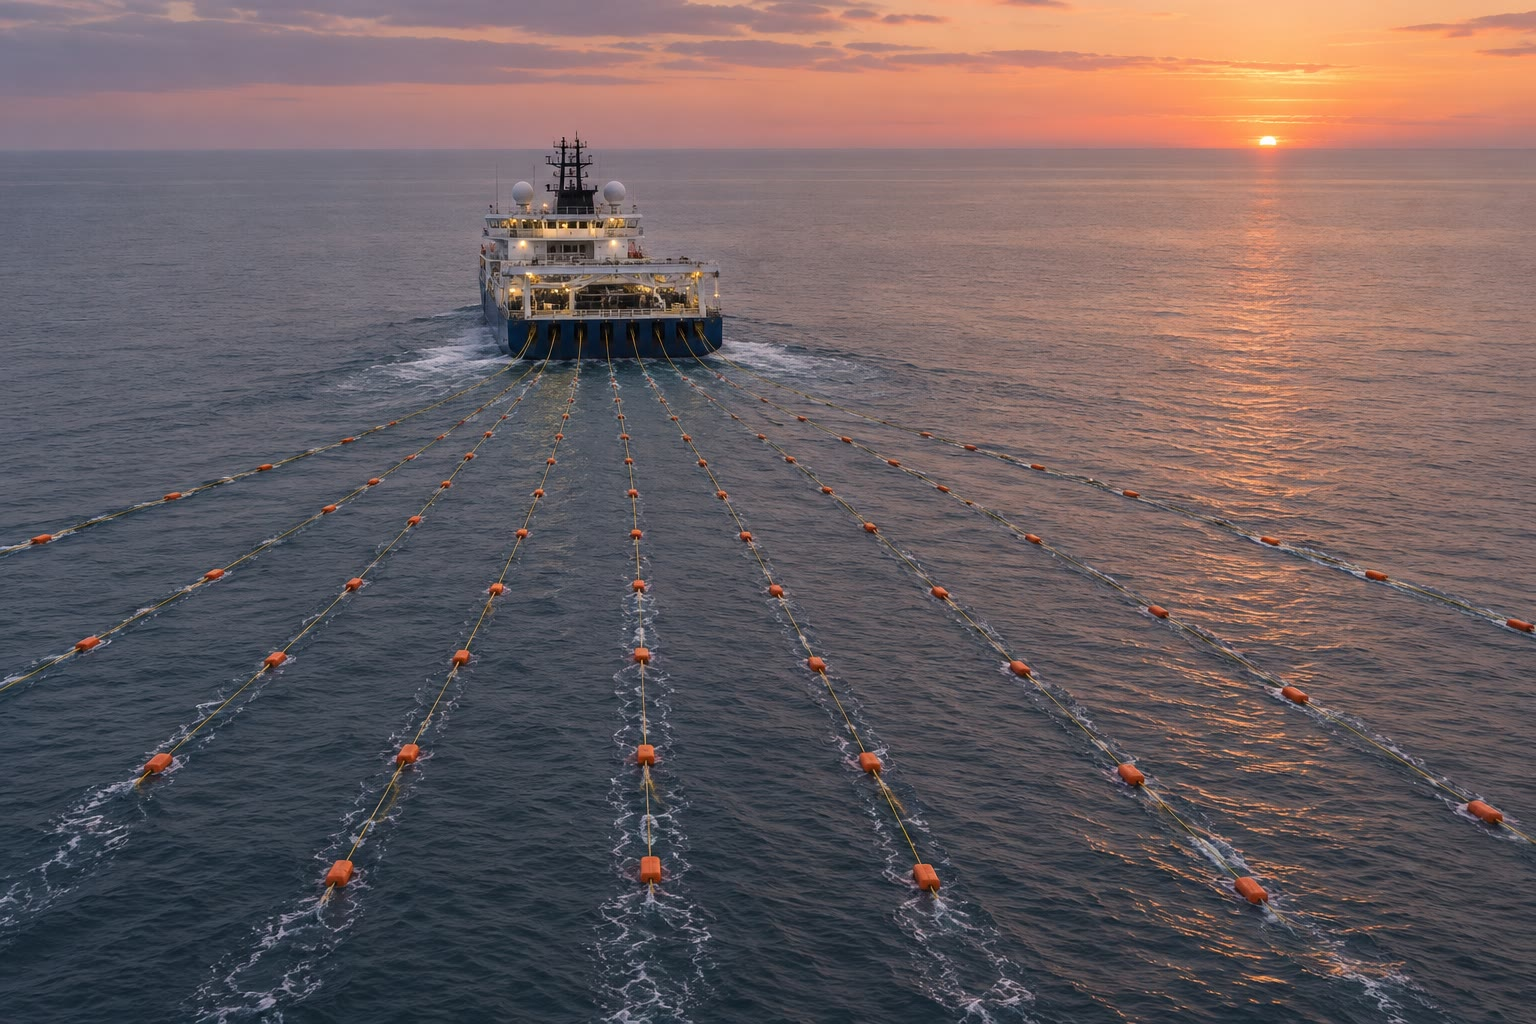
\includegraphics[width=\linewidth]{images/book5/ai/b3-streamer-vessel.jpg}

{\scriptsize Un navire de prospection sismique remorquant ses flûtes au crépuscule
(Illustration générée par IA.)}
\end{minipage}
\end{inthefield}

\section{Exercices}

\begin{exercise}[$\star$]\label{exo:b3:exploration-seismology:1}
La craie ($v = \qty{2500}{m.s^{-1}}$, $\rho = \qty{2.00}{g.cm^{-3}}$) repose sur des schistes argileux
(\qty{2300}{m.s^{-1}}, \qty{2.30}{g.cm^{-3}}), qui repose sur du calcaire
(\qty{4500}{m.s^{-1}}, \qty{2.60}{g.cm^{-3}}). Calculer les trois impédances acoustiques et
les coefficients de réflexion des deux interfaces. Quelle fraction
de l'énergie incidente le sommet du calcaire réfléchit-il~?
% ledger: mavko:velocities
\end{exercise}

\begin{exercise}[$\star$]\label{exo:b3:exploration-seismology:2}
Un réflecteur plat se trouve à \qty{800}{m} sous une couche de \qty{2000}{m.s^{-1}}.
Calculer $t_0$, le temps de réflexion à un déport de \qty{1000}{m}, et le \omterm{thm:b3:exploration-seismology:nmo}{retard normal}
correspondant ici, puis comparer ce résultat à l'approximation $x^2/(2v^2t_0)$.
\end{exercise}

\begin{exercise}[$\star$]\label{exo:b3:exploration-seismology:3}
Une flûte compte 240 voies espacées de \qty{12.5}{m}, et le navire tire tous les
\qty{25}{m}. Calculer l'intervalle des points milieux communs et l'\omterm{def:b3:exploration-seismology:cmp}{ordre de couverture}. Quel intervalle de tir
donnerait un \omterm{def:b3:exploration-seismology:cmp}{ordre de couverture} de 120~?
\end{exercise}

\begin{exercise}[$\star$]\label{exo:b3:exploration-seismology:4}
Pour une fréquence dominante de \qty{30}{Hz}, calculer la longueur d'onde et le
quart de longueur d'onde dans un grès de \qty{3000}{m.s^{-1}} et dans un calcaire de
\qty{4500}{m.s^{-1}}. Calculer le rayon de la première \omterm{def:b3:exploration-seismology:fresnel}{zone de Fresnel}
d'un réflecteur situé à \qty{1000}{m} de profondeur sous des roches de vitesse moyenne \qty{2800}{m.s^{-1}}.
\end{exercise}

\begin{exercise}[$\star\star$]\label{exo:b3:exploration-seismology:5}
Deux réflexions ont $t_0 = \qty{0.500}{s}$ et une \omterm{def:b3:exploration-seismology:velocities}{vitesse quadratique moyenne} de
\qty{2400}{m.s^{-1}}, et $t_0 = \qty{0.700}{s}$ avec une vitesse de \qty{2800}{m.s^{-1}}.
Calculer la \omterm{def:b3:exploration-seismology:velocities}{vitesse d'intervalle} et l'épaisseur de la couche comprise entre elles.
\end{exercise}

\begin{exercise}[$\star\star$]\label{exo:b3:exploration-seismology:6}
Un réflecteur plan a un pendage $\varphi$ dans le plan d'une ligne à points milieux communs, dans une couche
de vitesse $v$. (a) Montrer que $t(x)^2 = t_0^2 + x^2\cos^2\varphi/v^2$, où $t_0$ est
le temps à déport nul au point milieu. (Indice~: utiliser le symétrique du point milieu
par rapport au réflecteur.) (b) En déduire la \omterm{def:b3:exploration-seismology:velocities}{vitesse de sommation}, et la calculer pour
$v = \qty{2000}{m.s^{-1}}$ et $\varphi = \ang{12}$.
\end{exercise}

\begin{exercise}[$\star\star$]\label{exo:b3:exploration-seismology:7}
Une collection de traces à \omterm{def:b3:exploration-seismology:cmp}{point milieu commun}, d'\omterm{def:b3:exploration-seismology:cmp}{ordre de couverture} 60, présente un bruit indépendant, de même variance, sur chaque trace. De
quel facteur la \omterm{def:b3:exploration-seismology:stack}{sommation} élève-t-elle le rapport signal sur bruit~? De quel facteur
faut-il augmenter l'\omterm{def:b3:exploration-seismology:cmp}{ordre de couverture} pour le doubler à nouveau~?
\end{exercise}

\begin{exercise}[$\star\star$]\label{exo:b3:exploration-seismology:8}
Sur une section en temps à déport nul, dans une roche de \qty{3000}{m.s^{-1}}, une réflexion
remonte de \qty{0.40}{s} de temps double par kilomètre le long de la ligne. Convertir cette
pente en pendage apparent, puis calculer le pendage réel du réflecteur.
\end{exercise}

\begin{exercise}[$\star\star$]\label{exo:b3:exploration-seismology:9}
Convoluer la \omterm{def:b3:exploration-seismology:synthetic}{série de réflectivité} $r = (0, 0.3, 0, -0.2, 0)$ avec
l'ondelette à trois échantillons $w = (-0.5, 1, -0.5)$, échantillon par échantillon. Où sont situées les deux
réflexions, et se recouvrent-elles~?
\end{exercise}

\begin{exercise}[$\star\star\star$]\label{exo:b3:exploration-seismology:10}
Un profil de réfraction inversé sur une couche de \qty{1800}{m.s^{-1}} donne une
vitesse apparente dans le sens du pendage de \qty{2900}{m.s^{-1}} et une vitesse apparente à contre-pendage de
\qty{4400}{m.s^{-1}}. Calculer l'angle critique, le pendage et la vitesse du
réfracteur. Comparer la vitesse du réfracteur à la moyenne harmonique des deux vitesses
apparentes.
\end{exercise}

\begin{exercise}[$\star\star\star$]\label{exo:b3:exploration-seismology:11}
Dans la \cref{prop:b3:exploration-seismology:tuning}, une couche présente des coefficients de réflexion
$+R$ et $-R$. (a) Montrer que, pour $\Delta t \ll T$, le signal composé est environ
$R\,\Delta t\,w'(t)$, c'est-à-dire la dérivée temporelle de l'ondelette
pondérée par l'épaisseur en temps double de la couche. (b) Expliquer pourquoi une couche mince peut malgré tout être
détectée sans être résolue, et comment son épaisseur pourrait être estimée à partir de
son amplitude. (c) Deux couches de même roche, de 5 et \qty{10}{m} d'épaisseur, sont
imagées avec la même ondelette~: quel est le rapport de leurs amplitudes~?
\end{exercise}

\begin{exercise}[$\star\star\star$]\label{exo:b3:exploration-seismology:12}
Un diffuseur ponctuel se trouve à \qty{600}{m} sous la ligne, dans une roche de
\qty{3000}{m.s^{-1}}. (a) Écrire le temps à déport nul de sa diffraction en fonction de
la distance horizontale $x$ au point situé à son aplomb, et le calculer pour $x = 0$
et \qty{300}{m}. (b) Montrer que la diffraction est une hyperbole de la forme du \omterm{thm:b3:exploration-seismology:nmo}{retard normal}
avec la vitesse $v/2$, et expliquer pourquoi une diffraction est toujours plus courbée qu'une
réflexion de même temps au sommet. (c) Que fait la migration de cette diffraction~?
\end{exercise}

\section{Problème~: une ligne sismique à travers les collines de Varden}

\begin{problem}[{Problème du week-end --- réfraction, analyse des vitesses, conversion en
profondeur et migration le long de la coupe A--B des collines de Varden}]
\label{pb:b3:exploration-seismology:1}
% values: calc/ch02.py, from figdata seismic_model.py, refraction_dip.py, cmp_nmo.py
Une ligne sismique est tirée le long de la coupe A--B des collines de Varden, la région
couverte par les cartes géologiques des volumes précédents. Ses distances $s$ sont comptées
à partir de A le long de la ligne. La couverture, du sommet vers la base, est constituée de craie, de schistes argileux (\qty{100}{m}),
de calcaire (\qty{180}{m}) et de grès (\qty{120}{m}), reposant en discordance sur
un socle schisteux~; elle est plissée en un anticlinal et un synclinal et recoupée par
une faille normale.

\medskip
\noindent\textbf{Partie I --- Un dispositif de réfraction sur le flanc ouest.} Un dispositif de
\qty{1200}{m} est déployé entre les points de tir O ($s = \qty{300}{m}$) et E
($s = \qty{1500}{m}$), sur un terrain considéré comme horizontal. La craie et les schistes situés au-dessus du
calcaire sont traités comme une seule couche de vitesse $v_1 = \qty{2.40}{km.s^{-1}}$.
Les temps des ondes coniques relevés sur les enregistrements sont, de O vers E, \qty{425.2}{ms} à
\qty{800}{m} et \qty{486.1}{ms} à \qty{1200}{m}~; de E vers O,
\qty{372.4}{ms} à \qty{800}{m} et \qty{486.1}{ms} à \qty{1200}{m}.
\begin{enumerate}
  \item Calculer les deux vitesses apparentes. Quel tir est situé en amont du pendage~?
  \item Calculer l'angle critique et le pendage du réfracteur.
  \item Calculer la vitesse du réfracteur. De quelle roche s'agit-il~?
  \item Calculer les temps d'interception et les profondeurs perpendiculaires du
        réfracteur sous O et sous E.
  \item Convertir ces profondeurs en profondeurs verticales, puis vérifier le pendage à partir des deux profondeurs.
  \item Les schistes sous la craie sont plus lents que la craie. Comment le dispositif
        de réfraction les interprète-t-il, et comment biaise-t-il les profondeurs~?
\end{enumerate}

\noindent\textbf{Partie II --- Analyse de vitesse au CMP S.} Plus à l'est, le CMP S
se situe sur l'axe du synclinal, dans le compartiment abaissé de la faille, là où
les couches sont considérées comme horizontales. Quatre réflexions sont pointées à déport nul et à
\qty{600}{m}~:
\begin{center}
\small
\begin{tabular}{lcccc}
\hline
réflexion & 1 & 2 & 3 & 4 \\
$t_0$ (\unit{s}) & 0.4878 & 0.5748 & 0.6548 & 0.7348 \\
$t(\qty{600}{m})$ (\unit{s}) & 0.5437 & 0.6240 & 0.6887 & 0.7648 \\
\hline
\end{tabular}
\end{center}
\begin{enumerate}[resume]
  \item Calculer la vitesse NMO $V = x/\sqrt{t^2 - t_0^2}$ des réflexions 1
        et 2. Pourquoi la seconde est-elle plus petite que la première~?
  \item Calculer cette vitesse pour les réflexions 3 et 4.
  \item En prenant ces valeurs pour des \omterm{def:b3:exploration-seismology:velocities}{vitesses quadratiques moyennes}, calculer la \omterm{def:b3:exploration-seismology:velocities}{vitesse d'intervalle} de chaque
        couche par l'\omterm{thm:b3:exploration-seismology:dix}{équation de Dix}.
  \item Identifier les couches à partir de leurs vitesses, et nommer les quatre
        interfaces réflectrices.
  \item La réflexion 1 est la plus faible sur les enregistrements. Pourquoi~?
  \item Pourquoi les vitesses ont-elles été mesurées seulement sur les déports allant jusqu'à \qty{600}{m}
        alors que le dispositif atteint \qty{2}{km}~?
\end{enumerate}

\noindent\textbf{Partie III --- Conversion en profondeur et résolution.}
\begin{enumerate}[resume]
  \item Calculer le temps double passé dans chaque couche, puis son épaisseur.
  \item Calculer la profondeur de chaque interface réflectrice sous le sol. Comparer
        les épaisseurs des schistes, du calcaire et du grès avec les valeurs
        données plus haut.
  \item Calculer la vitesse moyenne du sol jusqu'au socle, et expliquer pourquoi
        la vitesse NMO de la réflexion 4 surestimerait la profondeur si on l'utilisait
        à la place.
  \item L'\omterm{def:b3:exploration-seismology:wavelet}{ondelette sismique} de la campagne culmine à \qty{30}{Hz}. Calculer la longueur d'onde dans
        les schistes et leur \omterm{def:b3:exploration-seismology:resolution}{épaisseur d'accord}, à la fois par la règle du quart de longueur d'onde
        et par $b = v/(5.2f)$ pour une \omterm{def:b3:exploration-seismology:wavelet}{ondelette de Ricker}. Les schistes sont-ils résolus~? À
        quelle fréquence mettrait-on les schistes en accord selon la règle du quart de longueur d'onde~?
  \item Calculer le rayon de la première \omterm{def:b3:exploration-seismology:fresnel}{zone de Fresnel} sur le socle, en prenant
        $\lambda$ à partir de la vitesse NMO de la réflexion 4.
\end{enumerate}

\noindent\textbf{Partie IV --- Migration et faille.}
\begin{enumerate}[resume]
  \item Près de la faille, la coupure du calcaire produit une diffraction
        dont le sommet est à \qty{0.550}{s}~; à \qty{200}{m} du sommet, le long de la ligne
        elle se trouve à \qty{0.5732}{s}. Écrire le temps de diffraction à déport nul et
        en déduire la vitesse moyenne au-dessus de la coupure.
  \item Calculer la profondeur de la coupure sous le sol.
  \item Sur le flanc est, la réflexion du sommet du calcaire de la section sommée
        remonte vers l'anticlinal de \qty{0.167}{s} de temps double par
        kilomètre, sous des roches de vitesse moyenne \qty{2.48}{km.s^{-1}}. Calculer son
        pendage apparent et son pendage réel.
  \item Une réflexion sur ce flanc est enregistrée à $t = \qty{0.655}{s}$. De combien,
        et dans quel sens, la migration la déplace-t-elle~?
  \item À travers la faille, la réflexion du sommet du socle saute de \qty{0.160}{s}~;
        le compartiment abaissé porte l'épaisseur supplémentaire de craie. Calculer le
        rejet vertical.
  \item Donner la profondeur de la discordance du socle sous le CMP S, à partir des
        \omterm{def:b3:exploration-seismology:velocities}{vitesses d'intervalle} de la partie II.
\end{enumerate}
\end{problem}
